%!TEX root = ../thesis.tex
%*******************************************************************************
%****************************** Fourth Chapter **********************************
%*******************************************************************************
\chapter[From discrete to continuum dislocation dynamics]{Role of weakest links and system-size scaling in multiscale modelling of stochastic plasticity \hyperref[paper:A2]{[O1]}} \label{chapter:weakest_link}

% **************************** Define Graphics Path **************************
\ifpdf
    \graphicspath{{Chapter4/Figs/Raster/}{Chapter4/Figs/PDF/}{Chapter4/Figs/}}
\else
    \graphicspath{{Chapter4/Figs/Vector/}{Chapter4/Figs/}}
\fi

In this study the intermittent local strain burst events involved in plastic deformation of crystalline materials will be investigated from a numerical and theoretical point of view. This approach differs completely from that of chapter \ref{chapter:in_situ}, where new technological ideas will be introduced to facilitate and improve the experimental examination of the avalanche-like behaviour in crystalline materials.

To better understand the physical basis of the phenomenon a minimal stochastic continuum plasticity model (SCPM) \nomenclature[z-SCPM]{SCPM}{stochastic contiuum plasticity model} is introduced, where the details of the microstructure of the dislocations are taken into account via a fluctuating local yield threshold which is one possibility to handle the question raised in section \ref{sec:disloc_sim_LDA} after \cref{eq:friction_stress_coeff}, namely the actual form of $\alpha$\footnote{The value $\alpha$ can be calulated by a kind of weighted average of the stress field induced by a dislocation, where the weights are coming from a specific linear combination of the two-particle dislocation-dislocation density function. Under specific assumptions one can consider the value of $\alpha$ to be constant, but due to its high sensitivity on the local dislocation arrangement, one can also envisage it as a fluctuating value around a mean value.}. In this published study (see point \hyperref[paper:A2]{O1} at chapter \ref{chapter:publications}) a method for determining the appropriate yield stress distribution in micron scale plasticity is presented. The distribution we propose is derived from lower scale DDD simulations which is combined with weakest link arguments. To demonstrate the success of the parameter-derivation in the microplastic regime, stress-strain curves obtained from both the SCPM and the lower.scale DDD models are presented. The two models behave identically in the thermodynamic limit and they are statistically equivalent shown by various scaling properties. The proposed technique can be adapted to different microstructures and also to amorphous materials according to our expectations.

\section{Introduction}
Understanding and modelling crystal plasticity requires multiscale approaches as the plasticity itself involves features of the specimen on multiple spatial and temporal scales from the smallest, atomic scales through the scales of crystal defects (point-like defects, dislocations or even dislocation patterns) and grain microstructure up to the specimen size. In a fortunate situation one can separate the size scales in the sense that at a given scale level lower phenomena are taken into account by only a restricted amount of parameters. Such scale linking is offered by the DDD and CDD approaches in crystal plasticity, an enticing possibility intensively studied \cite{Groma_2003_AM,PhysRevLett.114.015503,Hochrainer_2014_JMPS,POH2013913,LEVKOVITCH20067246,doi:10.1080/14786430600972921}. The main advantage of having descriptions on different levels is that difficulties appearing at lower levels can disappear on higher scales due to appropriate approximations chosen carefully. In the case of dislocations this difficulty on a lower level arises from the fact that dislocations interact via a long range force field, therefore in DDD simulations each pair-interaction must be taken into account leading to a disadvantageous scaling of the computational cost. This restricts simulations to only a couple of thousands of dislocations or dislocation segments. An appropriate CDD model might lift this restriction, where continuous density field quantities represent the dislocations, and the dynamics of dislocations is translated into coupled partial differential equations of these fields.

Continuum descriptions filter out spatial fluctuations below the the size scale of the mean dislocation spacing which play an important role of the intermittent strain bursts caused by dislocation avalanches \cite{doi:10.1080/14786430802132522,Dimiduk1188}. Such fluctuations may be negligible for bulk samples but certanly not for micron-scale specimens where they derange the prediction of formability causing a major challenge for material design \cite{Csikor251}. Spatial fluctuations may also increase average strength of specimens with dimensions reduced down to the micron scale or even below, a size effect observed in experimental investigation \cite{DIMIDUK20054065,Dimiduk1188,doi:10.1146/annurev-matsci-082908-145422}. One way to take into account the important physics of strain bursts is to extend CDD models by introducing a new stochastic component appearing in the differential equations.

Such SCPM was proposed in 2D\cite{1742-5468-2005-08-P08004}, where the stochastic component arises in a random component as the local yield stress of the material. This component is meant t account for the stress-fluctuations below the mean dislocation spacing which can be caused by formation and breaking of local jammed configurations such as narrow dislocation dipoles or junctions in 3D. The model discretises both time and space leading to a cellular automaton (CA) representation. The equations are solved in this framework and the plastic strain field is investigated thereafter. The stochastic nature of plasticity is successfully captured by the resulting model \cite{1742-5468-2007-04-P04013} which is also suitable for modelling the quasiperiodic oscillatory behaviour observed in micropillars at a low strain rate \cite{papanikolaou2012quasi}.

SCPMs were first introduced to study plasticity in amorphous materials \cite{0965-0393-2-2-001,PhysRevLett.89.195506}, where dislocations cannot play any role in the deformation. It is surprising, how such models can be also used in strongly different systems, namely in crystalline materials, to study plasticity. The basic assumptions which lead to usability of the similar models are:
\begin{enumerate}
\item The accumulation of plastic strain can be resolved into smaller events taking place in a localised region. These events decrease the on-site stress and cause a long-range stress-rearrangement in the sample with equivalent asymptotic properties.
\item A fluctuation in the local yield stress accounts for the disorder below the scale of resolution of the CA model .
\end{enumerate}

A version of the SCPM -- equivalent with the one used in this study -- was recently introduced to study avalanche phenomena in amorphous materials \cite{PhysRevE.84.016115,PhysRevE.88.062403,1742-5468-2015-2-P02011,PhysRevLett.116.065501}. The reason why equvivalent models can describe completely different materials lies in the concept that a local strain increment can be envisaged as an adequate Eshelby inclusion problem \cite{Eshelby376}. This can be realised both with or without dislocations resulting practically the same mathematical formula which explains the first point in the previous enumeration. The conceptional differences of the materials can be taken into account in the second point of the enumeration. As an example, in the works of \citet{PhysRevE.84.016115} and \citet{1742-5468-2005-08-P08004}, they both use a probabilistic distribution for the local yield stress but their actual form differs, as they intend to represent different microstructural features of the actual material, hence differ between crystalline and amorphous solids.

In this study a possible approach is presented 	how these parameters can be calibrated for the case of crystal plasticity. The role of the underlying lower-scale model is played by two types of 2D DDD models that have been investigated extensively in the past \cite{miguel2001intermittent,PhysRevLett.106.105501,ovaska2015quenched,1742-5468-2015-8-P08009}. A load-controlled quasistatic plastic deformation will be performed where the beginning and end of the avalanches can be well defined \cite{PhysRevLett.112.235501}. The microplastic regime will be in focus where no system-scale yielding occurs. It will be shown that Weibull distribution characterises the external stress at the event of first dislocation avalanche, and the mean stress at the $i$th avalanche follows a weakest link sequence from the same distribution. An in-depth statistical analysis will be also provided to show by scaling relations that both simulations of DDD and SCPM exhibit a smooth plastic response at not too large strains when the system size tends to infinity. With an appropriate choice of the other SCPM parameters its plastic response can be fitted to those obtained for DDD models at least in the microplastic regime, meaning they are statistically equivalent.

\section{Simulation models}
For the sake of simplicity only 2D models are considered in this chapter. To mimic an infinite crystal (or to avoid of introducing extra external conditions), toroidal periodic boundary conditions are used. We premise that the stress field of a dislocation is required under periodic boundary conditions. It can be found in the work of \citet{BAKO200622} based on the book of \citet{hirth1982theory}. For simplicity, the equations in this chapter uses the infinite-large limit form. Only the key features of the models will be discussed throughout this section as they have been used extensively in the literature.

\subsection{Stochastic continuum plasticity model} \label{sec:weakest_SCPM_description}
The SCPM used in our study is based on the pioneering work of \citet{1742-5468-2005-08-P08004} aiming of studying crystal plasticity at the micron scale. Their model considers a 2D plain strain situation where slip can only occur on one single slip system. Without loss of generality here we assume the plastic strain tensor to be of the form ${{\mathbf{\varepsilon }}^{{\text{pl}}}}\left( {\mathbf{r}} \right) = {\gamma ^{{\text{pl}}}}\left( {\mathbf{r}} \right) \cdot {\mathbf{M}}$, where ${\gamma ^{{\text{pl}}}}\left( {\mathbf{r}} \right)$ is the scalar plastic strain and ${\mathbf{M}} = \left( {{{\mathbf{e}}_x} \otimes {{\mathbf{e}}_y} + {{\mathbf{e}}_y} \otimes {{\mathbf{e}}_x}} \right)/2$. Not only the strain but also the local stress -- denoted by ${\tau _{{\text{loc}}}}\left( {\mathbf{r}} \right)$ -- is a scalar field quantity, as only the shear component plays a role.  In an infinite system the shear stress at a position $\mathbf{r}$ can be written as 
\begin{equation} \label{eq:weakest_tau_loc}
{\tau _{{\text{loc}}}}\left( {\mathbf{r}} \right) = {\tau _{{\text{ext}}}} + \left( {{G_{\rm{E}}} * {\gamma _{{\text{pl}}}}} \right)\left( {\mathbf{r}} \right),
\end{equation}
where ${\tau _{{\text{ext}}}}$ represents the remote boundary tractions, ${G_{\rm{E}}}\left( {\mathbf{r}} \right)$ is the elastic Green's function determined by the solution of the Eshelby inclusion problem \cite{Eshelby376} -- which also includes the details of the actual form of plastic deformation -- and the star $*$ denotes the spatial convolution. \Cref{eq:weakest_tau_loc} means that the local stress field consists of two parts: an external term influenced by the environment and an internal term generated by the inhomogeneous plastic deformation field. The stress and strain fields are discretised on a square lattice with directions parallel and perpendicular to the slip direction. The size of a cell in the lattice is $d$ in the dimensionless units described in appendix \ref{sec:dimensionless_units}, and the size of the whole lattice is $L \cdot d \times L \cdot d$ and different values for $L$ has been chosen to investigate the properties of the model as the system size tends to infinity. In this study $L=8,16,32,...,512$ were used. Space coordinates are discretised and the indices $i$ and $j$ are used to denote the coordinates where $x=i \cdot d$ and $y = j \cdot d$. The Green's function is also discretised, ${G_{\rm{E}}}\left( {i,j} \right)$, which gives the stress field caused by a plastic slip event at the origin, ${\gamma _{{\text{pl}}}}\left( {i,j} \right) = {\delta _{i0}}{\delta _{j0}}\Delta {\gamma _{{\text{pl}}}}$, where ${\delta _{kl}}$ is the Kronecker symbol and $\Delta {\gamma _{{\text{pl}}}}$ is the size of the plastic event. The elementary slip event is implemented by adding four dislocations with Burgers vectors $b{{\mathbf{e}}_{\mathbf{x}}}$, $b{{\mathbf{e}}_{\mathbf{y}}}$, $-b{{\mathbf{e}}_{\mathbf{x}}}$ and -$b{{\mathbf{e}}_{\mathbf{y}}}$ at the right, top, left and bottom sides to the cell that has to be deformed leading to a plastic deformation of $\Delta {\gamma _{{\text{pl}}}} = 2/d$. (Fig.~\ref{fig:weakest_elementary_slip_event} illustrates the procedure.) The stress value generated by these four dislocations is then calculated at cell $\left( {i,j} \right)$ and evaluated at the centerpoints of the cells. In the very centre this gives ${G_{\rm{E}}}\left( {0,0} \right)\Delta {\gamma _{{\text{pl}}}} =  - 4\Delta {\gamma _{{\text{pl}}}} =  - 8/d$. For the rest of the cells the result can be seen in Fig.~\ref{fig:weakest_greens_function} in the units of  $\left| {{G_{\rm{E}}}\left( {0,0} \right)} \right| \cdot \Delta {\gamma _{{\text{pl}}}}$. The Green's function describes the stress-redistribution in the sample, and in accordance with Newton's axiom, itself does not decrease or increase the average stress since $\sum\limits_{i,j = 0}^L {{G_{\rm{E}}}\left( {i,j} \right)}  = 0$.


\begin{figure}[htbp!] 
\centering    
\includegraphics[width=0.6\textwidth]{periodic_dipole_stress_field128x128symm_bin_dat_tilized_multiplot2}
\caption[Stress field of the elementary slip event]{The central part of the stress field of the elementary slip event, ${G_{\rm{E}}}\left( {i,j} \right) \cdot \Delta {\gamma _{{\text{pl}}}}$ in the units of $\left| {{G_{\rm{E}}}\left( {0,0} \right)} \right|\Delta {\gamma _{{\rm{pl}}}}$. System size: $L=128$. In the inset the part $\left[ { 0,2} \right] \times \left[ { 0,2} \right]$  is enlarged and the individual value of the stress of the cells are shown. The pattern has a fourfold symmetry which comes from the symmetric arrangement of the dislocations at four sides of the cell $\left( {0,0} \right)$.}
\label{fig:weakest_greens_function}
\end{figure}

The dislocation microstructure inside a cell determines the local flow stress, a fluctuating local threshold value which prevents plastic flow in case of too small local stresses, i.e., if for a given cell
\begin{equation} \label{eq:weakest_loc_equilibrium}
{\tau _{\rm{r}}}\left( {{\mathbf{r}},t} \right): = {\tau _{{\text{th}}}}\left( {{\mathbf{r}},t} \right) - \left| {{\tau _{{\text{loc}}}}\left( {{\mathbf{r}},t} \right)} \right| > 0
\end{equation}
holds (r for residual), then the cell is in equilibrium, the dislocations move neither on a continuum nor on the discrete level. When the inequality does not hold, the cell is active, it yields. The value of ${\tau _{{\text{th}}}}\left( {{\mathbf{r}},t} \right)$ is different from cell to cell, and its actual value is chosen from a given distribution, assigned first to each cell at the beginning of the simulation. This threshold value is an independent random variable for each cell and correlations between the cells are neglected which implies some non-controlled assumptions on the cell size. The values are taken from a Weibull distribution 
\begin{equation} \label{eq:weakest_weibull}
P\left( {{\tau _{{\text{th}}}}} \right) = \frac{\beta }{{{\tau _w}}}{\left( {\frac{{{\tau _{{\text{th}}}}}}{{{\tau _w}}}} \right)^{\beta  - 1}}{e^{ - {{\left( {{\tau _{{\text{th}}}}/{\tau _w}} \right)}^\beta }}}
\end{equation}
with shape parameter $\beta=1, 1.4, 2$ and scale parameter ${{\tau _w}}$. The threshold value of a cell is regenerated after each plastic deformation occurring at that cell. The plastic strain is considered homogeneous at the beginning of the simulation leading to 0 internal stress. The loading procedure is stress-controlled, starts from 0 and is increased quasi-statically: First it is increased until a single site violates \cref{eq:weakest_loc_equilibrium}, that is, it gets activated activated. The local strain is then increased by $\Delta {\gamma _{{\text{pl}}}}$ in the active cell and a new ${{\tau _{{\text{th}}}}}$ value is assigned from the very same Weibull distribution used at the beginning. The change in the local strain changes the internal stress not only in the active cell, but also elsewhere, due to the non-localness of the Green's function. The change caused by the plastic event is calculated according to \cref{eq:weakest_tau_loc}. Activated cells are identified by \cref{eq:weakest_loc_equilibrium} and strain applied to those cells which violates the inequality referenced and internal stress is recalculated. This search, strain generation and internal stress recalculation is done over and over again as long as the inequality violated at least for one cell. An avalanche is defined by the sum of the plastic events occurring at this given external stress.

Extremal dynamic is considered, meaning, if more the one cell violates the local equilibrium at once, strain is applied to that cell first for which ${\tau _r}$ is the smallest negative number, and then the recalculation of the internal stress field is done. When no more cells are activated, the avalanche is closed and the external stress is increased again to that value where at least one cell violates the inequality initiating a new avalanche.

The total strain $\gamma$ is defined as $\gamma  = \left\langle {{\gamma _{{\text{pl}}}}} \right\rangle $, where $\left\langle  \bullet  \right\rangle $ denotes the spatial average.

\begin{figure}[htbp!] 
\centering    
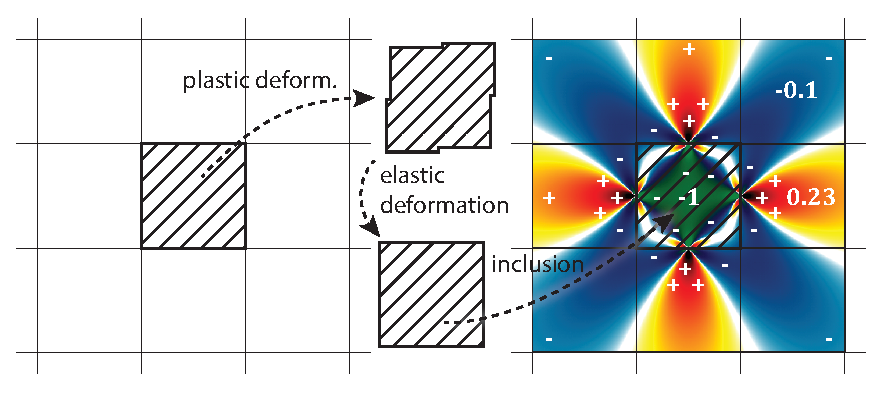
\includegraphics[width=0.6\textwidth]{arrangement}
\caption[Sketch of elementary slip event]{The sketch shows the elementary slip event. Four dislocations are placed on the edges of the active cell which causes a plastic strain $\Delta {\varepsilon ^{{\rm{pl}}}} = \Delta {\gamma ^{{\rm{pl}}}} \cdot {\bf{M}} = \Delta {\gamma ^{{\rm{pl}}}} \cdot \left( {{{\bf{e}}_x} \otimes {{\bf{e}}_y} + {{\bf{e}}_y} \otimes {{\bf{e}}_x}} \right)/2$. Then the cell is elastically deformed to fit back into its original position. The stress field this procedure generates can be calculated on the basis of the generalised Eshelby's inclusion problem and is equivalent with the stress field of the four dislocations. This deformation procedure creates the stress field shown on Fig.~\ref{fig:weakest_greens_function}. The stress field of the four dislocations are evaluated at the centerpoints of the cells.}
\label{fig:weakest_elementary_slip_event}
\end{figure}


\subsection{Discrete dislocation dynamics}
Two types of DDD models are used in this study. A time and space continuous one and one where both time and space are discretised.

\subsubsection{Time continuous DDD}
The model called time-continuous DDD (TCDDD) is the conventional DDD model, widely used in the literature. Here we consider $N$ straight parallel edge dislocations in the same slip system describing the easy slip regime of a face centered cubic (FCC) \nomenclature[z-FCC]{FCC}{face centered cubic} crystal at low temperatures (no climb and cross-slip, only glide).

There are two types of dislocations considered differing only in their Burgers vector, ${\mathbf{b}} = \left( {b,0} \right)$ and ${\mathbf{b}} = \left( {-b,0} \right)$. The first is called a positive dislocation $s=1$ and latter as a negative one $s=-1$. Equal amount of positive and negative dislocations are considered (no excess dislocations). The simulation space is square shaped with sides parallel and perpendicular to the Burgers vector and since they are edge dislocations, they move parallel to the $x$ axis, therefore only the shear component of the stress tensor plays a role in the EOM of the dislocations. An individual dislocation at the origin induce an anisotropic shear stress field at the position ${\mathbf{r}}$ as 
\begin{equation}
{\tau _{{\text{ind}}}}\left( {\mathbf{r}} \right) = x\frac{{{x^2} - {y^2}}}{{{{\left( {{x^2} + {y^2}} \right)}^2}}} = \frac{{\cos \left( \phi  \right)\cos \left( {2\phi } \right)}}{r},
\end{equation}
where $\left( {r,\phi } \right)$ are polar coordinates and units are omitted in agreement with appendix \ref{sec:dimensionless_units}.

The acting external stress is considered to be homogeneous and strong damping is considered due to phonon drag (over-damped motion) therefore the EOM of the $i$th dislocation, being at position ${{\mathbf{r}}_i} = \left( {{x_i},{y_i}} \right)$ is given by 
\begin{equation} \label{eq:weakest_EOMx}
\frac{{d{x_i}}}{{dt}} = {s_i}\left[ {{\tau _{{\text{ext}}}} + \sum\limits_{j = 1;j \ne i}^N {{s_j}{\tau _{{\text{ind}}}}\left( {{{\mathbf{r}}_i} - {{\mathbf{r}}_j}} \right)} } \right]
\end{equation}
and
\begin{equation} \label{eq:weakest_EOMy}
\frac{{d{y_i}}}{{dt}} = 0.
\end{equation}
where this latter means the absence of climb.

At the beginning of the simulations values are assigned independently to both $x$ and $y$ coordinates from a uniform distribution leading to no initial spatial correlations between the dislocations. Then \cref{eq:weakest_EOMx} is numerically solved and iterated until each dislocation reaches equilibrium defined by a low enough non-zero value limit for the average absolute velocity. This initial transient was not considered in the forthcoming evaluation as it belongs only to the generation of the initial state and time measurement is started from the end of relaxation.

In the following phase the plastic response of the system is simulated due to applied load. The external stress is increased at a constant rate till the system reaches the $v\left( t \right) > {v_{\rm{c}}}$ condition. The system is considered to be in the state of an avalanche if $v\left( t \right) > {v_{\rm{c}}}$ holds and during an avalanche the external stress is kept constant implementing a quasistatic load-controlled procedure. (The procedure is illustrated in Fig.~\ref{fig:weakest_DDD_lavina_def}.)

  
\begin{figure}[htbp!] 
\centering    
\includegraphics[width=0.6\textwidth]{bako_ddd_lavina_def}
\caption[Loading protocol and avalanches in a DDD]{On an individual realisation of a DDD simulation the quasistatic loading procedure is illustrated. If the average velocity $v$ of the dislocations (signed with their Burgers vector) is below a threshold value $v_{{\rm{c}}}$, the rate of the external stress is chosen as a constant value. If the $v>v_{{\rm{th}}}$, the external stress is kept constant.}
\label{fig:weakest_DDD_lavina_def}
\end{figure}

Plastic activity in this model has two different aspects.
\begin{enumerate}
\item During avalanches the strain rate is high and weakly depends on the external driving rate.
\item Between avalanches the strain rate is non-zero and proportional to the external stress rate and the deformation is quasireversible.
\end{enumerate}
The border of this two regimes is well defined by a carefully chosen value of ${{\dot v }_{\rm{c}}}$.

In agreement with appendix \ref{sec:dimensionless_units}, system size can be expressed by the number of dislocations as $L = {N^{0.5}}$ which explains the choice of the system sizes, chosen as $L=8,\,11.31,\,16,\,22.63,\,32$. For each system size large number of statistically equivalent realisations were taken ($3000,\,2000,\,800,\,300$ and $180$ respectively). For numerical reasons narrow enough dislocation dipoles were removed, but the introduction of this artificial length scale did not affect the phenomena investigated according to our verification.


\subsection{Cellular automaton DDD} \label{sec:weakest_CADDD}
The CADDD model is very similar to the continuous one introduced above but two restrictions are introduced which fasten up the simulation considerably.
\begin{enumerate}
\item Space is discretised into a square lattice with a cell size of $\delta$ and directions along the $x$ and $y$ axes. Dislocations can only jump from cell to a neighboring one in the $x$ direction. Only one dislocation can occupy a cell: the second dislocation of the same sign is not allowed to step to the same cell and dislocations with opposite signs annihilate each other if they are in the same cell. A very fine mesh was defined, more precisely, only every $128 \times 128$th cell was populated at the beginning.
\item Time is also discretised using the following dynamics. The acting stress $\tau$ is evaluated at both right and left edges of the cells which contain a dislocation. If the stress is positive at the right side or negative at the left side, a step towards the given direction of the stress leads to a $\Delta E \sim \;\left| \tau  \right|\delta $ decrease in the elastic energy, where $\tau$ denotes the stress at the given edge. Dislocation with such property is called active dislocation. At each time step the active dislocation with the highest possible $\Delta E$ is identified and moved by one cell in the direction determined by the largest energy drop. If none of the dislocations is active at a given time, then the external stress is increased until it is large enough to activate one, which means a quasistatic load-controlled procedure just as in the other two models.
\end{enumerate}
Like in TCDDD, simulations are started from an uncorrelated random dislocation distribution followed by an initial relaxation. The speed-up due to this technique has two main reasons.
\begin{enumerate}
\item Some details on the dynamics are erased due to the rough space and time steps.
\item The finite number of possible pair-interactions can be precalculated and stored in the memory. 
\end{enumerate}
With the introduction of this CA DDD model it becomes possible to identify the effect of the chosen dynamics -- i.e.\ extremal with CA or overdamped with continuous -- on the numerical results obtained. However, comparison is limited at the small deformation and time scales as the discrete steps corrupt the dynamics of the small avalanches and also affect the quasireversible regime observed in TCDDD, as the the motion of a dislocation either belongs to an avalanche or either is not presented at all. This is, however, not a major issue as long as macroscopic deformation, avalanche statistics and stress-strain curves are investigated.

  
\begin{figure}[htbp!] 
\centering    
\includegraphics[width=0.6\textwidth]{stress_strain_sketch}
\caption[Stress-strain curve sketch]{Sketch of the external stress-strain curves obtained from the SCPM and DDD models. The curve is made of only steps, therefore the stress and strain information on each sequence (${\tau ^{\left( i \right)}}$ and ${\gamma ^{\left( i \right)}}$, respectively) describes the whole curve.}
\label{fig:weakest_stress_strain_sketch}
\end{figure}

\section{Numerical results} \label{sec:weakest_numerical_results}
In this section the simulation results are presented and analysed for the SCPM first, and then for the two types of DDD models simultaneously. For each model the results are presented in the following order:
\begin{enumerate}
\item For each model the stress-strain curves show a step-like behaviour and differ among realisations for the same model. Therefore the average of the stress-strain curves will be in focus first.
\item Then the fluctuation in the plastic response will be evaluated.
\item Individual strain bursts are investigated then, started with the stress sequence denoted by ${\tau ^{\left( k \right)}}$. (See Fig.~\ref{fig:weakest_stress_strain_sketch} for the definition of ${\tau ^{\left( k \right)}}$.)
\item And finally the strain sequence is analysed denoted by ${\gamma ^{\left( k \right)}}$. The way the numbers are assigned and a short outlook is presented in Fig.~\ref{fig:weakest_stress_strain_sketch}.
\end{enumerate}
From now on $\tau$ will denote the external stress.

\subsection{SCPM} \label{sec:weakest_SCPM}
Three scalar parameters of the SCPM were under investigation.
\begin{enumerate}
\item The $\beta$ shape parameter of the Weibull distribution (see \cref{eq:weakest_weibull}) characterizing the local yield stress distribution.
\item The strain increment at each elementary slip deformation denoted by $\Delta {\gamma _{{\text{pl}}}}$.
\item The scale parameter $\tau_w$ characterising the average strength of a cell $\left\langle {{\tau _{{\text{th}}}}} \right\rangle $. For Weibull distributions with $\beta$ values considered in this study, ${\tau _w} \approx 1.1 \cdot \left\langle {{\tau _{{\text{th}}}}} \right\rangle $ holds.
\end{enumerate}
One of the last two parameters can be always eliminated by measuring the stress in units of $\left\langle {{\tau _{{\text{th}}}}} \right\rangle $ and strain in the units of $\Delta {\gamma _{{\text{pl}}}}$, which defines a nondimensional coupling constant $I = \Delta {\gamma _{{\text{pl}}}}/\left\langle {{\tau _{{\text{th}}}}} \right\rangle $. According to our choice $\left\langle {{\tau _{{\text{th}}}}} \right\rangle $ was set to 1 and $\Delta {\gamma _{{\text{pl}}}}$ was the variable. Where it is not stated otherwise, $\beta=1.4$ and $\Delta {\gamma _{{\text{pl}}}} = 1/4$ were used.

\subsubsection{Average stress-strain curve} \label{sec:weakest_scpm_av_ssc}


\begin{figure}[htbp] 
  \centering
  \begin{subfigure}[b]{0.44\textwidth}
    \includegraphics[width=\textwidth]{stress_strain_curve_scaled}
    \caption{The effect of the shape parameter $\beta$. The power-law region is consistent with the $\langle \tau \rangle = \gamma^{1/\beta \zeta}$ relation predicted by \cref{eq:weakest_spm_stress_expect_manyexp} with $\zeta=1$. No size effect is observed, apart from the smallest plastic regimes with large scatter in ${\tau _{{\text{th}}}}$ ($\beta=1$), the curves collapse.}
    \label{fig:weakest_avg_stress_strain_SCPM_beta}   
  \end{subfigure}                  \hspace{0.01\textwidth}
  \begin{subfigure}[b]{0.53\textwidth}
    \includegraphics[width=\textwidth]{stress_strain_scaling_SCPM}
    \caption{The effect of $\tau_w$ and $\Delta \gamma^\text{pl}$ at $\beta=1.4$ and $L=128$. According to the scaling collapse shown in the inset the average stress-strain curves obey $\langle \tau \rangle = \tau_w^{1.32} (\Delta \gamma^\text{pl})^{-0.32} f(\gamma \tau_w^{-0.5} (\Delta \gamma)^{-0.5})$ with a suitable function $f$.\\ \\}
    \label{fig:weakest_avg_stress_strain_SCPM_I}
  \end{subfigure}
  \caption[Averaged stress-strain curves for the SCPM]{The averaged stress-plastic strain curves for the SCPM. In Fig.~(a) different values for the shape parameter $\beta$, while in Fig.~(b) different $\Delta {\gamma _{{\text{pl}}}}$ were used. In each case for small strains the curves follow a power-law, then saturate.}
  \label{fig:weakest_avg_stress_strain_SCPM}
\end{figure}

The stress-strain curves of the individual realisations were averaged at given strain values. This means that at a given strain value $\gamma$ the different values of the corresponding external stress were averaged. Fig.~\ref{fig:weakest_avg_stress_strain_SCPM_beta} shows the averaged stress-strain curve for different $\beta$ values and system sizes on a double logarithmic scale. The figure shows that the microplastic regime is described by a power law, 
\begin{equation} \label{eq:weakest_SCPM_stress_strain_scale}
\left\langle \tau  \right\rangle \left( \gamma  \right) = {\tau _1}{\gamma ^\alpha }
\end{equation}
over several orders of magnitude where $\tau_1$ is a constant and the exponent $\alpha$ depends on the shape parameter $\beta$ of the Weibull distribution. The fitted values of $\alpha$ along with other scale parameters obtained from this and the other two models can be found in \cref{tab:weakest_example}. The curves show no size effect, i.e.\ for a given $\beta$ the curves for different $L$ overlap, justifying that no size scaling was introduced in \cref{eq:weakest_SCPM_stress_strain_scale}. For plastic strains $\gamma \gtrsim 1$ the stress reaches a plateau due to infinitely large avalanches signaling the onset of continuous plastic flow.

Fig.\ref{fig:weakest_avg_stress_strain_SCPM_I} shows the role of $\Delta {\gamma _{{\text{pl}}}}$ and ${\tau _w}$. It was mentioned that only $I = \Delta {\gamma _{{\text{pl}}}}/{\tau _w}$ is the independent parameter. This feature can be seen for simulations with parameters $\left( {\Delta {\gamma _{{\text{pl}}}},{\tau _w}} \right) = \left( {1/2,2} \right),$ $\left( {1,4} \right)$ and $\left( {2,8} \right)$. By dividing the plastic strain by ${\Delta {\gamma _{{\text{pl}}}}}$ and the stress by ${\tau _w}$ the curves collapse for each of the individual realisation, therefore their averaged curve too at a mathematical precision.

It can be also seen in the figure that the curve depends on the specific choice of the parameters (for different value of $I$), but according to the inset, if the stress and strains are rescaled by ${\tau _w}$ and $\Delta {\gamma _{{\text{pl}}}}$, the curves collapse into a mastercurve with a specific scaling of the parameter $I$.


\subsubsection{Fluctuations in the plastic response}


\begin{figure}[htbp!] 
  \centering
  \begin{subfigure}[b]{0.48\textwidth}
    \includegraphics[width=\textwidth]{scaled_cumulative_external_stress_probability_at_0-007813_def}
    \caption{$\gamma  = 0.008$}
    \label{fig:weakest_stress_distrib_scpma}   
  \end{subfigure}          
%  \begin{subfigure}[b]{0.48\textwidth}
%    \includegraphics[width=\textwidth]{scaled_cumulative_external_stress_probability_at_0-01563_def}
%    \caption{$\gamma  = 0.016$}
%    \label{fig:stress_distrib_scpmb}   
%  \end{subfigure}             
  \begin{subfigure}[b]{0.48\textwidth}
    \includegraphics[width=\textwidth]{scaled_cumulative_external_stress_probability_at_0-03125_def}
    \caption{$\gamma  = 0.032$}
    \label{fig:weakest_stress_distrib_scpmc}
  \end{subfigure}
  \caption[Fluctuations in the plastic response for the SCPM]{The cumulative stress distributions at different deformation values for the SCPM are shown. As system size increases the width of distributions shrink, that is, stress fluctuations disappear for large samples. By multiplying a kind of effective external stress (which can be obtained as the external stress decreased by a certain value) with a power of the system size curves can be fitted with a normal distribution (dashed line) as seen in the insets.}
  \label{fig:weakest_stress_distrib_scpm}
\end{figure}

For each of the realisations the stress-strain curve is a staircase-like function as sketched in Fig.~\ref{fig:weakest_stress_strain_sketch}, but the averaging described above makes from the ensemble of these functions a smooth one hiding the underlying details. To recover this fluctuation the cumulative distribution function (CDF) \nomenclature[z-CDF]{CDF}{cumulative distribution function} of the stresses at a given strain for different realisations is measured and denoted by ${\Phi _\gamma }\left( \tau  \right)$. The wider this curve is the larger the scatter of the external stress is which are measured for different realisations. For bulk samples the individual stress-strain curves are identical meaning that there is no fluctuation in the external stress, therefore tending to larger values with the system size one expects the width of ${\Phi _\gamma }\left( \tau  \right)$ to shrink. As seen in Fig.~\ref{fig:weakest_stress_distrib_scpm} for all strains $\gamma$ the measured ${\Phi _\gamma }\left( \tau  \right)$ curves indeed tend towards a step function as the system size increases. The stress-strain curve of a bulk material is expected to become the $\left\langle \tau  \right\rangle \left( \gamma  \right)$ curve since there is no relevant size effect observed. This also implies that the step function the ${\Phi _\gamma }\left( \tau  \right)$ CDF tends towards must be located at the given value of $\left\langle \tau  \right\rangle \left( \gamma  \right)$. It is noted that the ${\Phi _\gamma }\left( \tau  \right)$ curves for different system sizes crosses each other in the very same point. This property may hide a connection between the system parameters not revealed in this study.


All the insets in Fig.~\ref{fig:weakest_stress_distrib_scpm} show that curves collapse after scaling the stresses by the system size around $\left\langle \tau  \right\rangle \left( \gamma  \right)$. Moreover the curves (see later section \ref{sec:weakest_theory_stress_sequence} and \cref{eq:weakest_spm_stress_expect_large_i}) can be fitted by a normal distribution 
\begin{equation} \label{eq:weakest_stress_distrib}
{\Phi _\gamma }\left( \tau  \right) = \frac{1}{2}\left[ {1 + {\text{erf}}\left( {\frac{{\tau  - \left\langle \tau  \right\rangle \left( \gamma  \right)}}{{c{L^{ - \theta }}}}} \right)} \right],
\end{equation}
where $c$ is an appropriate constant and $\theta $ is the exponent characterising the system size dependence on the stress fluctuations. It was found that the no size effect can be indentified on the stress-strain curve in which case $\theta =1$ is expected. Our findings are in good agreement with this expectation as $\theta  = 1 \pm 0.05$ was found.

Previously, a shifted Weibull distribution was used to fit ${\Phi _\gamma }\left( \tau  \right)$ onto the results for 2D and 3D DDD and as well as micropillar compression data \cite{ISPANOVITY20136234}. A normal distribution, however, has fewer parameters and is in good agreement with the theoretical arguments presented later in section \ref{sec:weakest_theory_stress_sequence}.

\subsubsection{Stress sequence}

In this and the upcoming sections the stress and strain sequences ${\tau ^{\left( i \right)}}$ and ${\gamma ^{\left( i \right)}}$ will be in focus, because they play a key role in the simple plasticity model to be introduced in section \ref{sec:weakest_simple_plasticity_model}. First the cumulative distribution ${\Phi ^{\left( 1 \right)}}$ of ${\tau ^{\left( 1 \right)}}$ (the external stress at first event) will be considered. In the SCPM the plastic strain is initially homogeneous (e.g.\ zero) everywhere, therefore until the first event the local stress is also homogeneous and equal to the applied external stress everywhere according to \cref{eq:weakest_tau_loc}. As a result the distribution of the external stress at the occurance of the first plastic event must be a Weibull distribution with shape parameter $\beta$ and scale parameter ${\tau _w} \sim {L^{ - 2/\beta }}$ (for explanation see section \ref{sec:weakest_theory_stress_sequence}). According to Fig.~\ref{fig:weakest_tau_i_scpma} ${\Phi ^{\left( 1 \right)}}$ indeed follows well the corresponding Weibull distribution, and the curves for different system sizes overlap if the stress is rescaled by ${L^{2/\beta }}$.

\begin{figure}[htbp!] 
  \centering
  \begin{subfigure}[b]{0.48\textwidth}
    \includegraphics[width=\textwidth]{plotting_cumulative_prob_at_ext_stress_scaled}
    \caption{The cumulative distributions $\Phi^{(1)}$ of the first activation stress $\tau^{(1)}$ are plotted. The scaling collapse for different system sizes is obtained by rescaling the stress by $L^{2/\beta}$. The corresponding Weibull distributions (given by \cref{eq:weakest_spm_stress_cumul}) are also plotted with black lines.}
    \label{fig:weakest_tau_i_scpma}   
  \end{subfigure}          \hspace{0.01\textwidth}
  \begin{subfigure}[b]{0.48\textwidth}
    \includegraphics[width=\textwidth]{scaled_mean_stress_at_ith_avalanche_1_1_4_2}
    \caption{The average stress sequence $\langle \tau^{(i)} \rangle$ is plotted. The curves are proportional with $i^{1/\beta}$ and the ones corresponding to different system sizes collapse if stresses are rescaled by $L^{2/\beta}$, in accordance with \cref{eq:weakest_stress_sequence_average}.\\ \\}
    \label{fig:weakest_tau_i_scpmb}   
  \end{subfigure}             
  \begin{subfigure}[b]{0.46\textwidth}
    \includegraphics[width=\textwidth]{deviation_of_stress_at_ith_avalanche_1_1_4_2}
    \caption{STD of the stress sequence $\delta \tau^{(i)}$. The curves are consistent with \cref{eq:weakest_stress_sequence_std}.}
    \label{fig:weakest_tau_i_scpmc}
  \end{subfigure}
  \caption[Stress sequences for the SCPM]{The analysis of the stress sequence for different shape values $\beta=1, 1.4, 2$ and system sizes for the case of SCPM. The findings led to the simple plasticity model introduced in section \ref{sec:weakest_simple_plasticity_model}. The model prediction is plotted in each subfig with black lines.}
  \label{fig:weakest_tau_i_scpm}
\end{figure}

Fig.~\ref{fig:weakest_tau_i_scpmb} and Fig.~\ref{fig:weakest_tau_i_scpmc} plot the average stress sequence $\left\langle {{\tau ^{\left( i \right)}}} \right\rangle $ and its standard deviation (STD) \nomenclature[z-STD]{STD}{standard deviation} $\delta {\tau ^{\left( i \right)}}$, respectively. For a given shape value $\beta$ the curves collapse for small $i$ values when the stress is rescaled by ${L^{2/\beta }}$. The mastercurves follow power laws,
\begin{equation} \label{eq:weakest_stress_sequence_average}
\left\langle {{\tau ^{\left( i \right)}}} \right\rangle  = {\tau _0}{\left( {\frac{i}{{{L^\eta }}}} \right)^{1/\beta }},
\end{equation}
\begin{equation} \label{eq:weakest_stress_sequence_std}
\delta {\tau ^{\left( i \right)}} = \frac{{{\tau _0}}}{{{i^{1/2}}}}{\left( {\frac{i}{{{L^\eta }}}} \right)^{1/\beta }},
\end{equation}
where the value of $\eta $ is estimated by visual analysis and $\eta =2.0\pm0.05$ is found.



\subsubsection{Strain sequence}


\begin{figure}[htbp!] 
  \centering
  \begin{subfigure}[b]{0.48\textwidth}
    \includegraphics[width=\textwidth]{plotting_deformation_at_ith_aval_1_1_4_2}
    \caption{The averaged strain sequences can be scaled together with an appropriate transformation of the ordinate.}
    \label{fig:weakest_gamma_i_scpma}   
  \end{subfigure}           \hspace{0.01\textwidth}
  \begin{subfigure}[b]{0.48\textwidth}
    \includegraphics[width=\textwidth]{plotting_deformation_deviation_at_ith_aval_1_1_4_2}
    \caption{The STD at each index value can also scaled with the same factor as for the sequence.}
    \label{fig:weakest_gamma_i_scpmb}   
  \end{subfigure}             
  \caption[Analysis of the strain sequences for SCPM]{Strain sequences from the SCPM. The strain $\gamma^{(i)}$ measured at the $i$th strain burst for different system sizes and $\beta$ values. The curves follow \cref{eq:weakest_strain_sequence_average} and \cref{eq:weakest_strain_sequence_std} (solid lines) with $\zeta=1 \pm 0.05$ and $\xi=2 \pm 0.1$. }
  \label{fig:weakest_gamma_i_scpm}
\end{figure}


The strain sequence shows similar properties to the stress sequence. The averaged curve and its deviation can be seen in Fig.~\ref{fig:weakest_gamma_i_scpm}. For small $i$ values both $\left\langle {{\gamma ^{\left( i \right)}}} \right\rangle $ and $\delta {\gamma ^{\left( i \right)}}$ follow power laws, 
\begin{equation} \label{eq:weakest_strain_sequence_average}
\left\langle {{\gamma ^{\left( i \right)}}} \right\rangle  = {s_0}\frac{{{i^\zeta }}}{{{L^\xi }}},
\end{equation}
\begin{equation} \label{eq:weakest_strain_sequence_std}
\delta {\gamma ^{\left( i \right)}} = \frac{{{s_1}}}{{{i^{1/2}}}}\frac{{{i^\zeta }}}{{{L^\xi }}},
\end{equation}
where values for $\zeta $ and $\xi $ are obtained by visual inspections: $\zeta  = 1.0 \pm 0.05$ and $\xi  = 2.0 \pm 0.1$. We found that both $\zeta $ and $\xi $ are insensitive to the exponent $\beta$ but ${{\gamma ^{\left( i \right)}}}$ and $\delta {\gamma ^{\left( i \right)}}$ themselves are sensitive, therefore $s_0$ and $s_1$ too. It means that the size of individual avalanches vary significantly in different cases.


\subsection{DDD models}
\subsubsection{Average stress-strain curve}

The average stress-strain curves for the DDD models were calculated the same way as for the SCPM detailed in section \ref{sec:weakest_scpm_av_ssc}. The stress-strain curves can be seen in Fig.~\ref{fig:weakest_avg_stress_strain_DDD} which show similar features to those obtained by the SCPM case, namely:
\begin{enumerate}
\item The microplastic regime is characterised by a power law with an exponent $\alpha  = 0.8 \pm 0.05$ (see \cref{eq:weakest_SCPM_stress_strain_scale}) and only a weak size effect can be seen.
\item This regime breaks down at $\tau  \approx 0.1$.
\item The curves saturate for large ($\gamma \gtrsim 10$) strains.
\end{enumerate}

\begin{figure}[htbp!] 
  \centering
  \begin{subfigure}[b]{0.48\textwidth}
    \includegraphics[width=\textwidth]{stress-average-at-gamma_v2}
    \caption{TCDDD}
    \label{fig:weakest_avg_stress_strain_TCDDD}   
  \end{subfigure}          
  \begin{subfigure}[b]{0.48\textwidth}
    \includegraphics[width=\textwidth]{avg_stress_strain_ca}
    \caption{CADDD}
    \label{fig:weakest_avg_stress_strain_CADDD}   
  \end{subfigure}             
  \caption[Analysis of the stress sequence for DDDs]{The average stress-strain curves of the DDD simulations. They follow a power-law until $\gamma \approx 0.1$, and saturate for large ($\gamma \gtrsim 10$) strains.}
  \label{fig:weakest_avg_stress_strain_DDD}
\end{figure}


Significant difference in the averaged stress-strain curves between the two DDD models arises only at large strains. In the work of \citet{1742-5468-2015-8-P08009} it is discussed, that the source of this discrepancy can be originated from artifact of the periodic boundary conditions. This phenomenon does not play any role at the initial part of the stress-strain curve, therefore it does not affect the statistical arguments presented in the followings, which is valid for small to medium strains only where the two DDD models exhibit similar behaviour.




\subsubsection{Fluctuation in the plastic response}

\begin{figure}[htbp!] 
  \centering
  \begin{subfigure}[b]{0.48\textwidth}
    \includegraphics[width=\textwidth]{TCDDD_stress-distrib-0_05}
    \caption{TCDDD; $\gamma = 0.05$}
    \label{fig:weakest_stress_distrib_ddd_TCDDD_005}   
  \end{subfigure}          
  \begin{subfigure}[b]{0.48\textwidth}
    \includegraphics[width=\textwidth]{TCDDD_stress-distrib-0_2}
    \caption{TCDDD; $\gamma = 0.2$}
    \label{fig:weakest_stress_distrib_ddd_TCDDD_02}   
  \end{subfigure}             
  \begin{subfigure}[b]{0.48\textwidth}
    \includegraphics[width=\textwidth]{CADDD_stress-distrib-0_05}
    \caption{CADDD; $\gamma = 0.05$}
    \label{fig:weakest_stress_distrib_ddd_CADDD_005}   
  \end{subfigure}          
  \begin{subfigure}[b]{0.48\textwidth}
    \includegraphics[width=\textwidth]{CADDD_stress-distrib-0_2}
    \caption{CADDD; $\gamma = 0.2$}
    \label{fig:weakest_stress_distrib_ddd_CADDD_02}   
  \end{subfigure}             
  \caption[Stress sequences for the DDDs]{The cumulative stress distributions $\Phi_\gamma$ at two different deformation levels $\gamma$ for the two DDD models. Scaling collapse can be obtained (see insets) by multiplying a kind of effective external stress (obtained by subtracting a certain value from the external stress) with a power of the system size, just as for the SCPM in Fig.~\ref{fig:weakest_stress_distrib_scpm}. The collapsed curves can be well fitted by an appropriate normal distribution (dashed lines).}
  \label{fig:weakest_stress_distrib_ddd}
\end{figure}



In Fig.~\ref{fig:weakest_stress_distrib_ddd} cumulative distributions ${\Phi _\gamma }\left( \tau  \right)$ of the stresses for different realisations at a given strain $\gamma$ are calculated and plotted, just as for the SCPM case, and the curves also share the similarities. Namely, the curves
\begin{enumerate}
\item tend to step functions as the system size increases,
\item intersect in a single point,
\item can be collapsed by scaling the stress with a certain power of the system size,
\item are well approximated by a normal distribution.
\end{enumerate}
As a consequence of the last point, \cref{eq:weakest_stress_distrib} holds with the proper exponent, here $\theta  = 0.8 \pm 0.05$, which means the system shows size dependency in this sense. Note that $0.8 = {\theta _{{\text{DDD}}}} < {\theta _{{\text{SCPM}}}} = 1$.




\subsubsection{The stress sequence}
\begin{figure}[htbp!] 
  \centering
  \begin{subfigure}[b]{0.48\textwidth}
    \includegraphics[width=\textwidth]{first-aval-stress_v3}
    \caption{The cumulative distribution $\Phi^{(1)}$ of the first activation stress $\tau^{(1)}$. Data collapse is obtained by plotting $\Phi^{(1)}$ as a function of $\tau L^{1.15}$ in the inset, plotted along a Weibull distribution with $\beta \approx 1.4 \pm 0.05$.}
    \label{fig:weakest_tau_i_tacdda}   
  \end{subfigure}           \hspace{0.01\textwidth}
  \begin{subfigure}[b]{0.48\textwidth} 
    \includegraphics[width=\textwidth]{i-th-aval-mean-stress}
    \caption{The average of the external stress $\tau^{(i)}$ at the \textit{i}th avalanche for different system sizes. The data are consistent with \cref{eq:weakest_stress_sequence_average} (solid lines) if $i\gtrsim3$ and $\langle \tau^{(i)}\rangle \lesssim 0.2$ and with $\beta = 1.4 \pm 0.05$ and $\eta = 1.6 \pm 0.1$.}
    \label{fig:weakest_tau_i_tacddb}   
  \end{subfigure}             
  \begin{subfigure}[b]{0.48\textwidth}
    \includegraphics[width=\textwidth]{i-th-aval-deviation-stress}
    \caption{The STD of the external stress $\tau^{(i)}$ at the \textit{i}th avalanche for different system sizes. The data are consistent with \cref{eq:weakest_stress_sequence_std} (solid lines) if $i\gtrsim3$ and $\langle \tau^{(i)}\rangle \lesssim 0.2$ and with $\beta = 1.4 \pm 0.05$ and $\eta = 1.6 \pm 0.1$.}
    \label{fig:weakest_tau_i_tacddc}
  \end{subfigure}
  \caption[Stress sequences for the TCDDD]{The analysis of the stress sequence $\tau^{(i)}$ for TCDDD simulations of different system sizes. Predictions according to the simple plasticity model introduced in \ref{sec:weakest_simple_plasticity_model} is plotted with black lines.}
  \label{fig:weakest_tau_i_tacdd}
\end{figure}


As mentioned in the description of the CADDD model \ref{sec:weakest_CADDD}, inter-avalanche events cannot be distinguished from small avalanches, therefore they ruin the statistics in investigating the stress and strain sequence at the low strain/stress limit. As a consequence, only the TCDDD model will be used in this analysis.

For the CADDD case, the analysis of the stress sequence can be seen in Fig.~\ref{fig:weakest_tau_i_tacdd}. According to Fig.~\ref{fig:weakest_tau_i_tacdda}, where the cumulative distribution ${\Phi ^{\left( 1 \right)}}$ of ${\tau ^{\left( 1 \right)}}$ (the external stress at the first plastic event) is plotted, a Weibull distribution with the proper shape parameter $\beta$ can be perfectly fitted onto the curve after collapsing the curves into a mastercurve (shown in the inset) via rescaling ${\tau ^{\left( 1 \right)}}$ by ${L^{\eta /\beta }}$ with parameters
\begin{equation} \label{eq:weakest_tcddd_beta}
  \beta  =  1.4 \pm 0.05,
\end{equation}
\begin{equation} \label{eq:weakest_tcddd_eta}
  \eta  =  1.6 \pm 0.1. 
\end{equation}

The rescaled $\left\langle {{\tau ^{\left( i \right)}}} \right\rangle $ and $\delta {\tau ^{\left( i \right)}}$ obey the same rule observed for SCPM in  \cref{eq:weakest_stress_sequence_average,eq:weakest_stress_sequence_std} and share the parameters as in \cref{eq:weakest_tcddd_beta,eq:weakest_tcddd_eta}.



\subsubsection{Strain sequence}

Figure \ref{fig:weakest_gamma_i_CADDD} shows some statistics on the strain measured at the $i$th event. The average strain $\left\langle {{\gamma ^{\left( i \right)}}} \right\rangle $ at the burst of the $i$th avalanche can be seen in Fig.~\ref{fig:weakest_gamma_i_CADDDa} and its STD in Fig.~\ref{fig:weakest_gamma_i_CADDDb}. The curves are in good agreement with \cref{eq:weakest_strain_sequence_average,eq:weakest_strain_sequence_std} estabilished for the SCPM first, but here the exponents were $\zeta  = 0.9 \pm 0.05$ and $\xi  = 1.5 \pm 0.1$.


\begin{figure}[htbp!] 
  \centering
  \begin{subfigure}[b]{0.48\textwidth}
    \includegraphics[width=\textwidth]{plotting_deformation_at_ith_aval_1_1_4_2}
    \caption{The averaged strain sequences can be scaled together with an appropriate transformation of the ordinate.}
    \label{fig:weakest_gamma_i_CADDDa}   
  \end{subfigure}           \hspace{0.01\textwidth}
  \begin{subfigure}[b]{0.48\textwidth}
    \includegraphics[width=\textwidth]{plotting_deformation_deviation_at_ith_aval_1_1_4_2}
    \caption{The STD at each index value can also scaled with the same factor as that of the sequence.}
    \label{fig:weakest_gamma_i_CADDDb}   
  \end{subfigure}             
  \caption[Analysis of the strain sequences for SCPM]{Strain sequences from the TCDDD. The strain $\gamma^{(i)}$ measured at the $i$th strain burst for different system sizes and $\beta$ values. The curves follow \cref{eq:weakest_strain_sequence_average}) and \cref{eq:weakest_strain_sequence_std} (solid lines) with $\zeta=0.9 \pm 0.05$ and $\xi=1.5 \pm 0.1$ for large enough system sizes. }
  \label{fig:weakest_gamma_i_CADDD}
\end{figure}


A summary of all the exponents introduced in this section can be found in Table~\ref{tab:weakest_example}.

\section{Simple plasticity model based on order statistics} \label{sec:weakest_simple_plasticity_model}

A simple plasticity model is introduced in this section based on the numerical results obtained in the previous sections of this chapter. In this model the deformation is stress controlled, elastic deformation is neglected and the stress-strain curve is a monotonous staircase function, which is completely characterised by the stress-strain sequence $\left( {{\tau ^{\left( i \right)}},{\gamma ^{\left( i \right)}}} \right)$ (for a sketch see \ref{fig:weakest_stress_strain_sketch}). The intention behind this picture is to model the stochastic feature of the plasticity investigated numerically in the previous section, therefore scaling forms in the model proposed will share the same notations as used at the evaluation of the results. A comprehensive overviewof the parameters can be found in Table.~\ref{tab:weakest_example}.

In this model we adopt the work of \citet{doi:10.1080/14786435.2014.932502} using a weakest link assumption to express the mean value of the stress sequence ${\tau ^{\left( i \right)}}$ and its STD. From the work of \citet{PhysRevLett.112.235501} we adopt a straightforward rule for the strain sequence to obtain the mean value and STD of the strain sequence in the TCDDD model too, where anomalous system size scaling has been observed. The combination of the stress and strain sequences gives a statistical prediction on the stress-strain curve which affirm our numerical results in section \ref{sec:weakest_numerical_results}. In our model the material can be decomposed into smaller units which interact via only the stress-field kernel. In the small deformation limit the plastic events are localised into a smaller portion of the material and the starting points of the avalanches are not affected by the deformation history.

In this model we will further assume, that
\begin{enumerate}
\item The Weibull-shaped activation threshold of a plastic events remains unchanged during plastic deformation.
\item The distribution of the avalanche size is stress independent.
\item By splitting up the stress-strain curve into small segments, in each interval many avalanches occur so that the summation of the strain sequences leads to a normal distribution according to the central limit theorem.
\end{enumerate}
The validity of the first two is questionable in a general case, especially for the SCPM where critical behaviour at high enough external stress can be observed, but can be accepted at the limit of small stresses, where avalanches are rather localised and not limited by the system size. The third assumption can be always legitimated if the system size $L$ is large enough.


\subsection{Stress sequence}  \label{sec:weakest_theory_stress_sequence}
The main idea of the SCPM is that plasticity occurs via irreversible local structural excitations which are activated at different stress values. This critical stress distribution $P\left( \tau  \right) = \frac{d}{{d\tau }}\Phi \left( \tau  \right)$ (the derivative of the cumulative distribution) represents the inhomogenities in the material at the resolution of the mesh size. During the stress increase the weakest sites are activated first, therefore only the $\tau  \to 0$ limit of this distribution plays a role at low strains. A reasonable proposition for this distribution \cite{doi:10.1080/14786435.2014.932502} is a power law as
\begin{equation} \label{eq:weakest_cumulative_is_power_law}
\Phi \left( \tau  \right) = {\left( {\frac{\tau }{{{\tau _0}}}} \right)^\beta }\quad {\text{if }}\tau  \to 0
\end{equation}
with $\beta \geqslant 1$. It is also assumed that the subsequent events are independent, i.e.\ no spatial correlations in the stress and plastic strain is present initially (at the low strain limit). If the number of independent sites is $M$, and $M \to \infty$, then the cumulative distribution of the $i$th stress value ${\tau ^{\left( i \right)}}$ follows a Weibull order statistics \cite{rinne2008weibull}, e.g.\ for the first value it is
\begin{equation} \label{eq:weakest_spm_stress_cumul}
{\Phi ^{\left( {1,M} \right)}}\left( {{\tau ^{\left( {1,M} \right)}}} \right) = 1 - \exp \left[ { - \frac{1}{M}{{\left( {\frac{{{\tau ^{\left( {1,M} \right)}}}}{{{\tau _0}}}} \right)}^\beta }} \right].
\end{equation}
The expected value of the $i$th event is given by
\begin{equation}  \label{eq:weakest_spm_stress_expect}
\left\langle {{\tau ^{\left( {i,M} \right)}}} \right\rangle  = \frac{{{\tau _0}}}{{{M^{1/\beta }}}}\frac{{\Gamma \left( {i + 1/\beta } \right)}}{{\Gamma \left( i \right)}} \approx {\tau _0}{\left( {\frac{i}{M}} \right)^{1/\beta }},
\end{equation}
and the STD by
\begin{equation}  \label{eq:weakest_spm_stress_deviat}
\delta {\tau ^{\left( {i,M} \right)}} = \sqrt {{{\left( {\frac{{{\tau _0}}}{{{M^{1/\beta }}}}} \right)}^2}\frac{{\Gamma \left( {i + 2/\beta } \right)}}{{\Gamma \left( i \right)}} - {{\left( {\frac{{\Gamma \left( {i + 1/\beta } \right)}}{{\Gamma \left( i \right)}}} \right)}^2}}  \approx \frac{{{\tau _0}}}{{{i^{1/2}}}}{\left( {\frac{i}{M}} \right)^{1/\beta }},
\end{equation}
where the approximation is exact in the limit when $i \to \infty$, $M \to \infty$ and $i/M \to 0$, and the error is less than $2\%$ if $i>5$ and if $M > 1000 \cdot i$ \citep[Sec. 6.1.47.]{abramowitz1964handbook}.

The findings are not restricted to only to the first few plastic events, but also applicable in the regime of order statistics, where $i/M=p$ finite. In the asymptotic limit, when $M \to \infty$ and $i/M=p$ is finite, the probability density function (PDF) \nomenclature[z-PDF]{PDF}{probability density function} of the $i$th smallest member drawn from $M$ samples -- whose CDF is $\Phi \left( \tau  \right)$ -- is normal distributed according to the central limit theorem, and its CDF is
\begin{equation} \label{eq:weakest_spm_stress_expect_large_i}
{\Phi ^{\left( {i,M} \right)}}\left( {{\tau ^{\left( {i,M} \right)}}} \right) = \frac{1}{2}\left[ {1 + {\text{erf}}\left( {\frac{{{\tau ^{\left( {i,M} \right)}} - \left\langle {{\tau ^{\left( {i,M} \right)}}} \right\rangle }}{{{\sigma ^{\left( {i,M} \right)}}}}} \right)} \right],
\end{equation}
in which the expected value is given by \cite{dasgupta2008asymptotic}
\begin{equation}
\left\langle {{\tau ^{\left( {i,M} \right)}}} \right\rangle  = {\Phi ^{ - 1}}\left( p \right): = \tau \left( p \right),
\end{equation}
and the deviation by
\begin{equation}
{\sigma ^{\left( {i,M} \right)}} = {\left( {\frac{{p\left( {1 - p} \right)}}{{M \cdot {{\left[ {\Phi '\left( {\tau \left( p \right)} \right)} \right]}^2}}}} \right)^{1/2}},
\end{equation}
where ${\Phi ^{ - 1}}\left( p \right)$ is the inverse of the CDF $\Phi \left( \tau \right)$ and $\Phi '$ is the derivative of the CDF, $\Phi ' = \frac{d}{{d\tau }}\Phi \left( \tau  \right)$. It was found that for small $p$ the CDF is $\Phi  \approx {\left( {\tau /{\tau _w}} \right)^\beta }$ which recovers \cref{eq:weakest_spm_stress_expect,eq:weakest_spm_stress_deviat}, hence extreme order statistics is applicable in the regime of finite $i/M$ too.

The connection between the number of sites $M$ and linear system size $L$ can be also discussed in the framework of this simple plasticity model. According to a common assumption, all sites are homogeneously distributed where plastic event can occur and their density does not depend on the system size. This leads to a $M \propto {L^d}$ connection, where $d$ is the physical dimension of  the system, in our case, $d=2$. In the DDD case results have shown anomalous size dependence which requires the refinement of this connection. Instead of $d$, a fractal dimension $\eta$ is introduced to describe the size dependence in the form
\begin{equation} \label{eq:weakest_anomalous_link_scaling}
M \propto L^\eta.
\end{equation}
Substituting this \cref{eq:weakest_anomalous_link_scaling} into \cref{eq:weakest_spm_stress_cumul,eq:weakest_spm_stress_expect,eq:weakest_spm_stress_deviat}, one gets
\begin{equation}
{\Phi ^{\left( 1 \right)}}\left( {{\tau ^{\left( 1 \right)}}} \right) =  1 - \exp \left( { - {{\left[ {\frac{1}{{{\tau _0}}}\frac{{{\tau ^{\left( 1 \right)}}}}{{{L^{\eta /\beta }}}}} \right]}^\beta }} \right),
\end{equation}
\begin{equation}
{\tau ^{\left( i \right)}} \approx  {\tau _0}{L^{ - \eta /\beta }} \cdot {i^{1/\beta }},
\end{equation}
and
\begin{equation}
\delta {\tau ^{\left( i \right)}} \approx  {L^{ - \eta /\beta }} \cdot {i^{1/\beta  - 1/2}}.
\end{equation}


\begin{table}[htpb]
\newcolumntype{L}[1]{>{\raggedright\let\newline\\\arraybackslash\hspace{0pt}}m{#1}}
\newcolumntype{C}[1]{>{\centering\let\newline\\\arraybackslash\hspace{0pt}}m{#1}}
\newcolumntype{R}[1]{>{\raggedleft\let\newline\\\arraybackslash\hspace{0pt}}m{#1}}
\centering
\caption{Summary of the exponents used in this study.}
\label{tab:weakest_example}
\begin{tabular}{L{1cm} L{4.0cm} C{2.1cm} C{1.7cm} C{2.0cm} C{2.0cm}}
\hline
Symbol & Description & Value predicted by theory & Value for SCPM & Value for TCDDD & Value for CADDD \\
\hline
$\beta$ & Characterizes threshold stress distribution, see \cref{eq:weakest_cumulative_is_power_law})  & - & $1.0$, $1.4$, and $2.0$\tablefootnote{This exponent is an input parameter for the SCPM model} & $1.4 \pm 0.05$ & - \\
$\eta$ & Describes the relation between the system size $L$ and the total number of links $M$, see \cref{eq:weakest_anomalous_link_scaling}) & - & $2.0 \pm 0.05$ & $1.6 \pm 0.1$ & - \\
$\zeta$ & Characterizes the strain sequence, see \cref{eq:weakest_spm_strain_expect}) & - & $1.0 \pm 0.05$ & $0.9 \pm 0.05$ & - \\
$\xi$ & Characterizes the system size dependence of the average avalanche size, see \cref{eq:weakest_gamma_step_average}) & $\eta \zeta$ & $2.0 \pm 0.1$ & $1.5 \pm 0.1$ & - \\
$\alpha$ & Exponent of the power-law characterizing the microplastic regime of the stress-strain curves, see \cref{eq:weakest_SCPM_stress_strain_scale}& $(\beta \zeta)^{-1}$ & $1.0\pm 0.05$, $0.7\pm 0.05$, and $0.5 \pm 0.05$ & $0.8\pm 0.05$ & $0.8 \pm 0.05$\\
$\theta$ & Exponent characterizing the system size dependence of the stress fluctuations, see \cref{eq:weakest_stress_distrib}) & $\eta/2$ & $1.0 \pm 0.05$ &  $0.8 \pm 0.05$ & $0.8 \pm 0.05$ \\
\end{tabular}
\end{table}

\subsection{Strain sequence}
The size of strain burst events may exhibit power-law distribution, revealed by recent experimental and numerical studies \cite{Dimiduk1188,doi:10.1080/14786430802132522,PhysRevLett.112.235501,miguel2001intermittent}. This distribution $P\left( {\Delta \gamma } \right)$ is upper bounded by ${\Delta {\gamma _u}}$, which can originate from the system size or other intrinsic bounds inherent in dynamics, and lower bounded by $\Delta {\gamma _l}$ due to the fact that a power law distribution with exponent smaller than $-1$ cannot be normalised around the singularity at 0. This boundary can be originated from e.g.\ the mean dislocation spacing -- which is orders of magnitude larger than the size of the dislocation core --, below which the individual dislocation motion may be the major source of plastic strain. Restricting our model above the lower  boundary, the size distribution can be written as
\begin{equation}
P\left( {\Delta \gamma } \right) = C \cdot \Delta {\gamma ^{ - {\tau _a}}} \cdot f\left( {\Delta \gamma /\Delta {\gamma _u}} \right)\quad {\text{if }}\Delta \gamma  > \Delta {\gamma _l}
\end{equation}
where ${\Delta \gamma }$ is the size of the strain increment, $C$ is a normalisation factor, ${{\tau _a}}$ is the avalanche size exponent and $f\left( x \right)$ is a cutoff function, which tends to $1$ for $x \to 0$ , and tends to $0$ for $x \to \infty$.

According to the work of \citet{PhysRevLett.112.235501}, $\tau^a \approx 1$ was found in the microplastic regime and $\Delta \gamma_u$ depends only weakly on the allied stress and exhibits anomalous system size dependence. In a work of \citet{1742-5468-2015-2-P02011}, for the SCPM case, $\tau_a \approx 1.35$ was found, and $\Delta \gamma_u$ diverges at a critical stress and exhibits regular system size dependence. The mean value of the strain size and its variance can be written in both cases as 
\begin{equation} \label{eq:weakest_gamma_step_average}
\left\langle {\Delta \gamma } \right\rangle  = \frac{{{s_0}}}{{{L^\xi }}},
\end{equation}
\begin{equation}  \label{eq:weakest_gamma_step_deviat}
\delta \left( {\Delta \gamma } \right) = \frac{{{s_1}}}{{{L^\xi }}},
\end{equation}
where $\xi$ is the exponent characterising the system size dependence, and $s_0$ and $s_1$ are constants depending e.g.\ on the applied stress. For the 2D DDD case, $\xi < 2$ represents anomalous scaling, where the total size of a plastic event depends on the system size. Value $\xi = 2$ correspond to normal scaling in 2D, as it was found for the SCPM.

In case one can assume the independence of the size of the subsequent events, central limit theorem for large enough $i$ values gives the value of the mean and variance in the form of 
\begin{equation} \label{eq:weakest_spm_strain_expect}
\left\langle {{\gamma ^{\left( i \right)}}} \right\rangle  = {i^\zeta }\left\langle {\Delta \gamma } \right\rangle  = {i^\zeta }\frac{{{s_0}}}{{{L^\xi }}}
\end{equation}
and
\begin{equation} \label{eq:weakest_spm_strain_deviat}
\delta {\gamma ^{\left( i \right)}} = {i^{\zeta  - 1/2}}\delta \left( {\Delta \gamma } \right) = \frac{{{i^\zeta }}}{{{i^{1/2}}}}\frac{{{s_1}}}{{{L^\xi }}}.
\end{equation}

\subsection{Stress-strain curves}
The possibility to express the stress-strain curve for one realisation from the individual ${\tau ^{\left( i \right)}}$ and ${\gamma ^{\left( i \right)}}$ sequences is given as they completely characterise the curve. For a given large enough value $i$ both follow a normal distribution according to \cref{eq:weakest_spm_stress_expect,eq:weakest_spm_stress_deviat} and to \cref{eq:weakest_spm_strain_expect,eq:weakest_spm_strain_deviat}. By inverting $\left\langle {{\gamma ^{\left( i \right)}}} \right\rangle \left( i \right)$ and substitute the value $i$ into ${\tau ^{\left( i \right)}}$ and using the approximation 
\begin{equation}
\left\langle {{\tau ^{\left( i \right)}}} \right\rangle \left( \gamma  \right) \approx {\tau ^{\left( {{{\left\langle {{\gamma ^{\left( i \right)}}} \right\rangle }^{ - 1}}\left( \gamma  \right)} \right)}},
\end{equation}
one gets 
\begin{equation} \label{eq:weakest_spm_stress_expect_manyexp}
\left\langle \tau  \right\rangle \left( \gamma  \right) = \frac{{{\tau _0}}}{{s_0^{1/\left( {\beta \zeta } \right)}}}{L^{\left( {\xi /\zeta  - \eta } \right)/\beta }}{\gamma ^{1/\beta \zeta }}
\end{equation}
and 
\begin{equation} \label{eq:weakest_spm_stress_deviat_manyexp}
\delta \tau \left( \gamma  \right) = {\tau _2}{L^{\left( {\xi /\zeta  - \eta } \right)/\beta  - \xi /\left( {2\zeta } \right)}} \cdot {\gamma ^{\left( {1/\beta  - 1/2} \right)/\zeta }}
\end{equation}
with ${\tau _2} = {\tau _0}/s_0^{\left( {1/\beta  - 1/2} \right)/\zeta }$. In this approximation the stress-strain curve follows power law and has a system size dependence for all (large) $L$ values if $\left( {\xi /\zeta  - \eta } \right)/\beta  \ne 0$. To avoid this non-physical behaviour, 
\begin{equation}
\xi  = \zeta \eta
\end{equation}
must hold. In this case \cref{eq:weakest_spm_stress_expect_manyexp,eq:weakest_spm_stress_deviat_manyexp} have the form
\begin{equation}
\left\langle \tau  \right\rangle \left( \gamma  \right) \propto {\gamma ^\alpha }\quad \alpha  = 1/\beta \zeta 
\end{equation}
and
\begin{equation} \label{eq:weakest_spm_stress_deviat_oneexp}
\delta \tau \left( \gamma  \right) \propto {L^{ - \theta }}\quad \theta  = \eta /2.
\end{equation}
\Cref{eq:weakest_spm_stress_deviat_oneexp} says that with increasing system size the STD decreases since $\theta>0$ and one obtains a well-defined, system size independent curve in the $L \to \infty$ limit.

\section{Summary}
The main idea of our SCPM is that a crystalline material can be treated as an arrangement of independent smaller units, each characterised by a local flow threshold (i.e.\ activation stress of a local plastic strain event) accounting for the inhomogeneity of the underlying dislocation microstructure not taken into account completely on the continuum level. According to the weakest link theory, the PDF of the external stress ${\tau ^{\left( 1 \right)}}$ at the onset of the first activated plastic event must follow a Weibull distribution.

This idea was supported by the numerical results of the TCDDD model, where the PDF of ${\tau ^{\left( 1 \right)}}$ followed a Weibull distribution with a shape parameter $\beta$ independent from the system size. Moreover, the shape parameter not only determines the asymptotic behaviour of the PDF of the stress threshold for the individual units, which is a power low with an exponent of $\beta$, but also plays a central role in forming the stress-strain curve. Theoretical explanation of the value found for $\beta \approx 1.4$ is out of the scope of this study, but similar connection can be found in 3D DDD models and in micropillar compression tests too \cite{ispanovity2010submicron,ISPANOVITY20136234}, where the stress-strain curves are investigated and obtained that $\alpha  = 1/\left( {\beta \zeta } \right) = 0.8$. In the following chapter (chapter \ref{chapter:disorder})) the role of $\beta$ in ductility of disordered materials exhibiting strain softening will be presented.

For both the SCPM and the DDD models the stress sequence followed a power law, with and exponent $\eta$ characterising the system size dependence. For the case of SCPM $\eta \approx 2$ was found representing normal system size scaling, i.e.\ the number of sites $M$ which can be activated scales with the linear size of the system on the power of the system dimension, $M \propto L^2$. Whereas for DDD $\eta \approx 1.5$ was found, a significantly smaller number than the physical dimension of the system suggesting a fractal-like arrangement of the activated sites. This presumption can be checked by calculating the correlation integral $C\left( r \right)$ for the coordinates\footnote{The correlation integral $C\left( r \right)$ on a set of points gives the frequency that two points can be found within a smaller distance than $r$.} of the dislocation avalanches.\footnote{By the coordinates of an avalanche we took the coordinates of the first plastic event within the avalanche.} Figure~\ref{fig:corrlation_integral} shows this correlation integral for the SCPM and DDD model. It tells that for large enough $r$ values they can be approximated by a power law and the findings support our conjecture: for the SCPM case the place of plastic strains follows a $r^2$ dependence while for the DDD case the function goes as $r^{1.6}$, i.e.\ the plastic strains are indeed accumulated on a fractal pattern of the material. This is in good agreement with the work of \citet{weiss2003three}, which states that the sources of the accousic emission signals are located on a fractal layer, morever, the fractal behaviour in our DDD model could explain the long-range nature of the correlations observed in the work of \citet{PhysRevLett.112.235501} investigating 2D DDD system, however, the origin of this fractal phenomenon is out of the scope of this study.


\begin{figure}[htbp!] 
\centering    
\includegraphics[width=0.6\textwidth]{corr_int}
\caption[Coreelation integral]{The correlation integrals of the starting positions of the avalanches for the SCPM and TCDDD models are plotted on a log-log scale. For both cases the integral follows a power law $C\left( r \right) \propto {r^\eta }$, with $\eta \approx 2.0$ and $\eta \approx 1.6$, respectively. Power laws with these exponents are also plotted with solid black lines.}
\label{fig:corrlation_integral}
\end{figure}

It is important to note that the size effects found in this study are not in connection with those general phenomena observed in other samples, where size effects come from surface effects as dislocation pile ups or dislocations running out of the sample at free boundary, but represents the behaviour of bulk samples as we implemented periodic boundary conditions. This boundary condition may lead to nonphysical artifacts (e.g.\ Fig.~\ref{fig:weakest_avg_stress_strain_CADDD} shows inverse size effect for large strains) which can be handled with an appropriate modification of the boundary conditions \cite{1742-5468-2015-8-P08009}.

The theoretical models used in this study are capable of describing the microplastic regime of micron-scale samples. We also found that there are only two independent exponents, $\beta$ and $\eta$, which, on the one hand, represent microstructural details of the material, on the other hand, they are directly linked to macroscopic quantities. $\beta$ can be obtained from the microplastic regime of stress-strain curve identifying the exponent of the power law, while $\eta$ can be determined from the stress fluctuations of different samples. By measuring these parameters in a model or even in real experiments one can set up the SCPM to reflect the desired behaviour . Figure~\ref{fig:stress_strain_comparison} shows a well configured SCPM in order to give similar results at microplastic regime then what we got for the DDD models. The fact that the stress-strain curve of the SCPM follows well the curve obtained for DDD models at larger strains too does not necessarily hold relevance as the model doesn't capture the internal strain correlations observed in DDD models.

\begin{figure}[htbp!] 
\centering    
\includegraphics[width=0.6\textwidth]{stress_strain_comparison}
\caption[Stress-strain curve comparison]{The stress-strain curves obtained from the three different plasticity models. The parameters of the SCPM were: $\beta  = 1.4$, $\Delta {\gamma _{{\rm{pl}}}} = 6$ and ${\tau _w} = 2$.}
\label{fig:stress_strain_comparison}
\end{figure}

\section*{Notes in regard to the thesis}
In this study we demonstrated that the SCPM model introduced earlier is capable of describing the stochastic properties of materials in the microplastic regime. A simple plasticity model has been proposed which is founded on the subsequent plastic events of crystalline samples in the microplastic regime. A methodology was proposed to compare the results of the SCPM and DDD models, which is suitable to determine how the free parameters of the SCPM should be chosen in order to reproduce the behaviour observed in the lower level DDD simulations.

The SCPM introduced earlier is based on a continuum model using the self-consistent field approximation which neglects the initial correlations of dislocations and let them evolve only through the signed (excess) dislocation density. It is known that such system exhibit non physical behaviour, e.g.\ the energy of the dislocation system is not an extensive quantity. However, this model is still suitable to describe some properties of the stochastic phenomena observed in crystal plasticity and gives an idea how to handle correctly the appearing $C$ parameter occurring in the local flow stress introduced in the continuum model with local density approximation at \cref{eq:flow_stress}.

My specific contribution to this study was primarily based on the SCPM. Based on the description found in the work of \citet{1742-5468-2005-08-P08004} I implemented a model first which reproduces the same statistics. Our target was to run large number of simulations but due to our moderate computational resources an efficient and free software was needed. Therefore, I wrote the whole program in C++. I further extended the model with the possibility to chose a local flowstress distribution, the actual form of the interaction kernel $G_E$ and the size of the plastic event along some other details not mentioned so far. I performed all the analysis of the data and contributed in preparing the corresponding manuscript and in preparing the figures therein.

It was also mentioned that the validity of this SCPM is not restricted to crystalline materials only but can be also used in amorphous materials. A model essentially based on this implementation can be found in the next chapter \ref{chapter:disorder}.

\subsection*{Negative results}

The reason why many other parameters or details have been investigated lies in our initial goal, which was namely to investigate the size distribution of the avalanches and how the parameters of the SCPM modify it. I also tried to point out the non-depinning behaviour of dislocation avalanches with the SCPM developed but it turned out that either the size scale used is too small to verify our goal or this is not the case, i.e.\ dislocations/dislocation groups are pinned at each site and a critical stress (yield stress) indeed exists where infinite large event occurs. It was also desired to find an anomalous system size scaling but our efforts rewarded no success and to exclude the possibility, that it is due to the small system size, large system sizes were again desirable. To achieve larger system sizes than $512 \times 512$, a program code for GPU has been written in CUDA which gave the same results as the one written in C++ and due to the nature of GPGPU the simulation time scales favourably with the system size and already at the size of $1024 \times 1024$ runs faster then on CPU\footnote{performed on an architecture which costs the same amount of money}. Unfortunately the acquisition of such devices has been canceled and only further improvements in the CPU code moved forward the investigation of the influence of the system size. The sophisticated CPU code on larger systems still didn't produce the results desired which made me to focus on other properties of the model, i.e.\ how to correctly set up all the parameters introduced in this model instead of their effect on the avalanche size distribution and the critical behaviour.

During these trials we found the robustness of the model, i.e.\ how insensitive the exponents are\footnote{For example, the size distribution of the avalanches, which are also investigated in the work of \cite{Csikor251}.} to many details of the model. Just to mention a few I list some of those, which leaves the exponent $\tau$ in the size distribution $P\left( s \right) = C \cdot {s^{ - \tau }} \cdot \exp \left[ { - {{\left( {s/{s_0}} \right)}^2}} \right]$ of dislocation avalanches unchanged.
\begin{itemize}
\item The actual shape of the flowstress distribution is almost irrelevant for the value of $\tau$, as long as it has finite mean value. In general, they modify only $s_0$.
\item The main property of the interaction kernel is its long-rangeness. If the four dislocations are split up into smaller ones, or rearranged into other configuration, the long range stress field remains basically the same, and does not affect the exponent $\tau$.
\item The event size introduced as $\Delta \gamma$ has been deeply analysed. Let us imagine the following scenario. The local flowstress is small and the total stress acting on the cell is also small, but larger then the local flowstress. Now let us activate this cell. The size of the plastic event is finite and can happen that according to the elastic kernel shown in Fig.~\ref{fig:weakest_greens_function}, it decreases the local stress below 0 and initiate a plastic event with a size of $-\Delta \gamma$. To avoid this, two techniques were implemented.
\begin{enumerate}
\item We used adaptive size for the plastic event, i.e.\ the $\Delta {\gamma _{{\text{actual}}}}$ was chosen so to decrease the local stress until to 0 only (as it was done later in the study in chapter \ref{chapter:disorder}). Or, as an alternative, the size can be chosen from a distribution with a mean value of $\Delta {\gamma _{{\text{actual}}}}$.
\item Plastic flow with negative size was disallowed.
\end{enumerate}
The original solution and the two extensions all gave the same value for the exponent $\tau$ and did not play a role in the size distribution of the avalanches. Due to the possibility of the negative flow (plastic event with negative plastic strain) the strain-stress sequence can be non-monotonous, which phenomenon could be completely eliminated by the second extension. No other remarkable effect was revealed.
\end{itemize}

Although it could be hard to publish the negative results mentioned above, they also headed me to the right direction of investigations and gave good basis for further plans.